
% RUN in terminal (without bibliography):
% pdflatex -output-directory=/Users/salvatorpes/Desktop/LFEUI/text/proposta /Users/salvatorpes/Desktop/LFEUI/text/proposta/prop.tex

\documentclass{article}

\author{
    \begin{tabular}{rl}
        Estêvão Gomes (ist1102650) & Sofia Nunes (ist1102633) \\
        Pedro Curvo (ist1102716) & Salvador Torpes (ist1102474)
    \end{tabular}
}

\usepackage[style=numeric]{biblatex} % Choose your desired citation style
\addbibresource{../references/prop.bib} % Specify your .bib file

\usepackage[utf8]{inputenc}
\usepackage[english]{babel}
\usepackage[letterpaper,top=6mm,bottom=15mm,left=6mm,right=6mm,marginparwidth=1.55cm]{geometry}
\usepackage{multicol}
\usepackage{graphicx}
\usepackage{subcaption}
\usepackage{tabularx}
\usepackage{booktabs}
\usepackage{array}
\usepackage{makecell}
\usepackage{titlesec}
\usepackage{multirow}
\usepackage{amsmath}
\usepackage{makecell}
\usepackage{url}
\usepackage{csquotes}
\usepackage{caption}
\usepackage{enumitem}
\usepackage{textcomp}
\usepackage{pdflscape}
\usepackage{makeidx}
% \usepackage{tocbibind}
\providecommand{\tightlist}{\relax}
\usepackage{tocloft}
\renewcommand{\cftsecindent}{0em}
\renewcommand{\cftsubsecindent}{1em}
\renewcommand{\cftsecfont}{\bfseries}
\renewcommand{\cftsubsecfont}{\itshape}
\setlength{\cftsubsecnumwidth}{0em}

\usepackage[version=4]{mhchem}
\usepackage{hyperref} % Remove "pdftex" option here
\usepackage{float}
\usepackage{fancyhdr}
\usepackage{ragged2e}
\usepackage{xkeyval}
%\usepackage{minted}
%\usemintedstyle{manni}
\usepackage{listings}
\usepackage{amssymb}
\usepackage{bookmark}
\usepackage{hyperref}
\usepackage{cleveref}


\usepackage{xcolor}
\usepackage{tikz}

\usetikzlibrary{positioning}
\usetikzlibrary{positioning, arrows.meta}
\usepackage{adjustbox}
\usepackage{sidecap}
\usepackage{graphicx}

\usepackage{tikz-3dplot}
\usepackage{pgfplots}
\usetikzlibrary{calc, 3d, arrows}



\usetikzlibrary{shapes.geometric, arrows}


% \lstset{
%     language=Python,
%     basicstyle=\ttfamily,
%     keywordstyle=\color{blue},
%     commentstyle=\color{gray},
%     stringstyle=\color{orange},
%     numbers=left,
%     numberstyle=\tiny,
%     numbersep=5pt,
%     showspaces=false,
%     showstringspaces=false,
%     breaklines=true,
%     frame=tb,
%     framexleftmargin=2em,
%     xleftmargin=2em,
% }


%\usepackage{fontspec}

%\setmonofont{Fira Code}

\fancyhf{}
\cfoot{\thepage}
\fancyhf{} % Clear all header and footer fields
\renewcommand{\headrulewidth}{0pt} % Remove the header rule line
\cfoot{\thepage} % Set the page number in the center of the footer

\pagestyle{fancy} % Apply the fancy page style

\setlength\columnsep{20pt}

\renewcommand{\familydefault}{\sfdefault}

\newenvironment{Figure}
  {\par\medskip\noindent\minipage{\linewidth}}
  {\endminipage\par\medskip}

\makeatletter
\newenvironment{figurehere}
{\def\@captype{figure}}
{}
\makeatother

\hypersetup{
  colorlinks,
  linkcolor=blue,
  anchorcolor=black,
  citecolor=cyan,
  filecolor=cyan,
  menucolor=cyan,
  urlcolor=cyan,
  bookmarksopen=true,
  bookmarksnumbered=true
}

\makeindex


\title{\vspace{-13mm}
\includegraphics[width=15mm,scale=3]{../images/IST_Logo.png}\\ \vspace{5mm}
LFEUI - Investigation Proposal \\ {\fontsize{24}{16}Detection of Li in Technological Materials through Nuclear Reactions} \vspace{-0mm}}
\date{November 2023}

\usepackage{sansmathfonts}
\usepackage[T1]{fontenc}
\usepackage[OT1]{fontenc}

\titleformat{\section}{\normalfont\large\bfseries}{\thesection}{1em}{}


\setlist[enumerate]{itemsep=3pt}

\begin{document}

\renewcommand{\arraystretch}{1.5}
\setlength{\columnseprule}{0.4pt}
\tdplotsetmaincoords{70}{110} % Set the viewing angle
\newcolumntype{M}[1]{>{\centering\arraybackslash\vspace{#1}}m{0.5\linewidth}<{\vspace{#1}}}
\newcolumntype{C}[2]{>{\centering\arraybackslash\vspace{#1}\rule{0pt}{#1}\hspace{0pt}}m{#2}}
\newcolumntype{w}[1]{>{\centering\arraybackslash}m{#1}}

\renewcommand*\familydefault{\sfdefault} %% Only if the base font of the document is to be sans serif

\maketitle

\vspace{-8mm}


\hrulefill

% \begin{center}
%   \textbf{\Large Abstract}
% \end{center}

\vspace{-0.1cm}
\begin{abstract}
  \par In the following document we present a proposal for a scientific research being developed at CTN Lisbon in December 2023.
  Our work consists of the detection of $\ce{^7Li}$ in two different samples through nuclear reactions.
  This document describes the time required for the project as well as it's goals, theoretical background, experimental technique, safety considerations and expected results.
  In addition, we also present a brief description of the experimental set-up.
\end{abstract}
\vspace{-0.1cm}

\hrulefill


\begin{multicols}{2}

% \tableofcontents

\section{Proposal Summary}

\paragraph{Goal}

Our main goal is to develop a scientific research project alongside three senior investigators from CTN
(Centro Tecnológico e Nuclear), Rodrigo Mateus, Rui Silva and Norberto Catarino. 

Our project will be focused on the detection of Li in technological materials through nuclear reactions.
The main motivation for this project is to study and develop a detection technique for elements such as Li with
high sensitivity.

\paragraph{Scientific Background}

This detection method is based on the nuclear reaction between the element we want to detect ($\ce{^7Li}$) and a proton, as follows:

\begin{equation}
  \ce{^7Li + ^1H -> ^8Be -> 2\alpha}
\label{eq:reaction}
\end{equation}

The reaction results in the production of a $\ce{^8Be}$ nucleus which then rapidly decays into two alpha particles. These are the particles we detect.

According to the incident proton's energy and the scattering angle of the detectors ($\theta = 165 $ degrees) we were able to use the NRA Calculator \cite{NRAEnergyCalc} to calculate the energy of the alpha particles resulting from the reaction as well as it's $Q$ value:

\begin{equation}
\begin{split}
  E_{\alpha_1} &= 7.65320 \text{ MeV} \\
  E_{\alpha_2} &= 10.89305 \text{ MeV} \\
  Q &= 17.34625 \text{ MeV}
\end{split}
\label{eq:energies}
\end{equation}

The formula this website uses to compute the energies is on the page 382 of the book \cite{krane1988}.

\section{Experimental technique}

\paragraph{Set-up}

The experimental set-up consists of a Tandem accelerator, a beam line with an electromagnet and a chamber with both the samples and the detectors.
The accelerator produces a beam of protons with a kinetic energy of up to 5 MeV which is deviated by the electromagnet and hits the sample. 
The electromagnets deflect particles with different angles according to their charge-to-mass ratio and, with that, allows us to remove any unwanted particles from the beam and only let the protons pass through.
The detectors used are silicon detectors - these detect charged particles through the ionization they produce in the silicon.

In addition, they are connected to a electronic system that amplifies the signal and sends it to a computer where we
can see the results.

The beam line is under a vacuum of around $10^{-7}$ mbar in order to avoid the protons colliding with other particles and losing energy. 
They reach the sample with the specified kinetic energy and cause a nuclear reaction whose products are the charged particles detected.
We aim to analyze the energy spectrum of these particles.

The following diagram shows the experimental set-up:
Note: We use a tandem accelerator, so the image should have 2 tubes inside the accelerator.

\begin{center}
  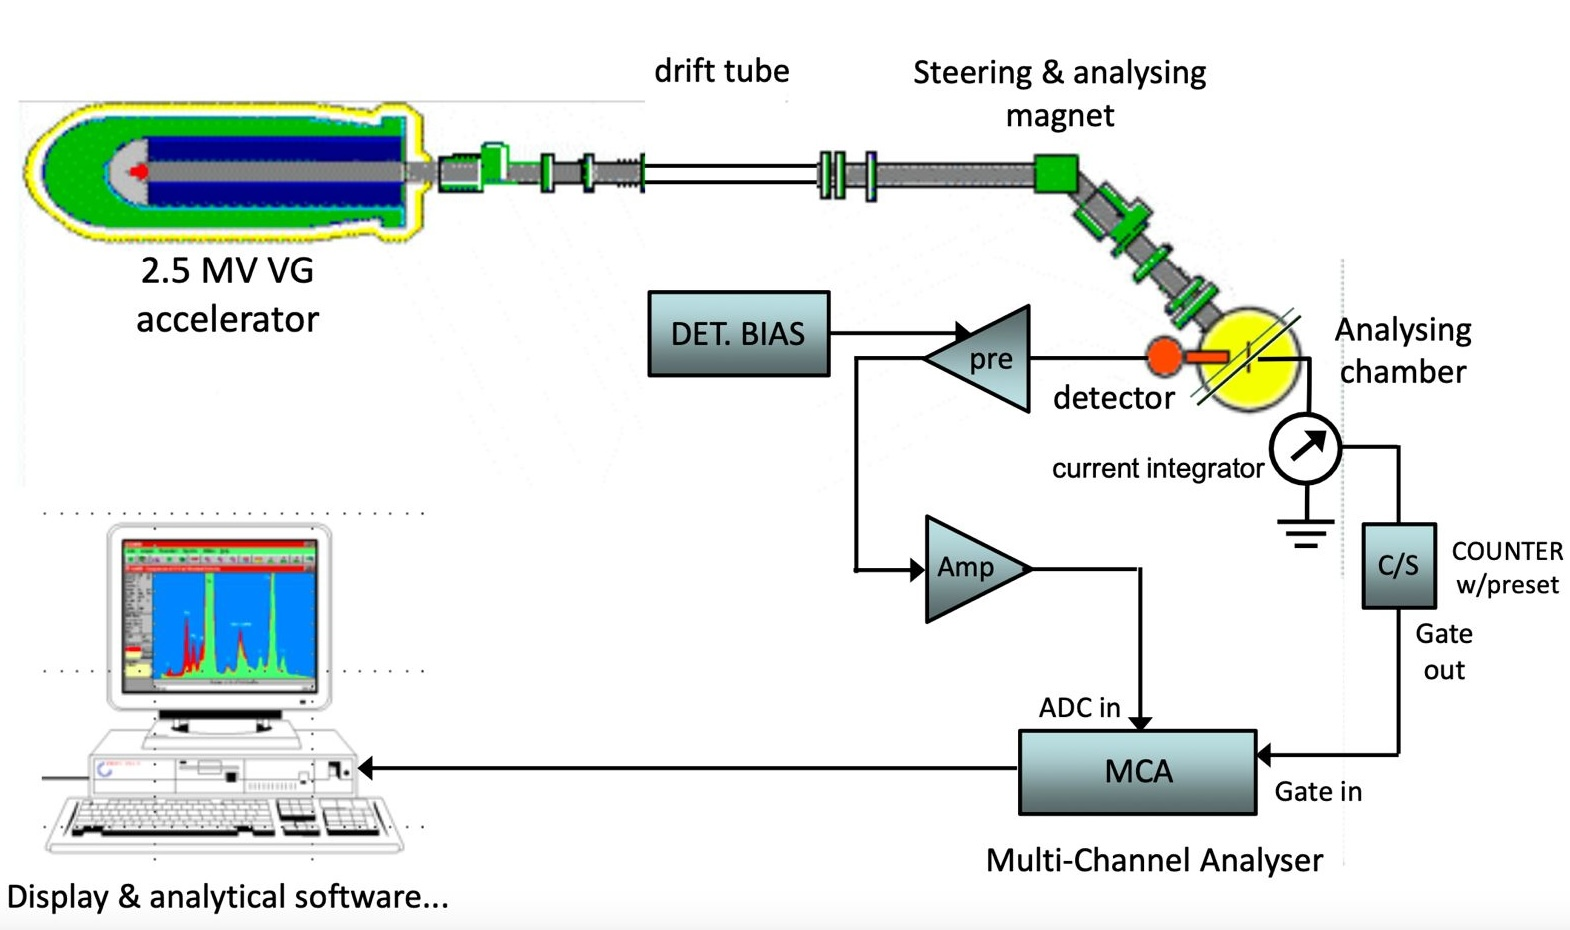
\includegraphics[width=0.95\linewidth]{../images/scheme.jpeg}
  \captionof{figure}{Experimental set-up.}
  \label{setup}
\end{center}

\paragraph{Samples}

We are going to work with two different Lithium-7 samples: one of them is a glass sample composed of silicon, boron and
lithium and the other one is a implant sample, which is a thin layer of lithium implanted in a silicon substrate.

\paragraph{WorkPlan}

Obtaining the energy spectrum of the alpha particles resulting from the reaction between the protons and the samples will
evolve the following steps:

\begin{enumerate}
  \item Accelerator Startup;
  \item Calibration of the detectors with a sample of known composition;
  \item Obtaining the energy spectrums of both samples with the appropriate beam energy;
  \item Analysis of the results.
\end{enumerate}

\paragraph*{Beam Energy}

In order to choose the energy of the beam we need to take into account the cross section of the reaction between the the protons and the Li-7.
We collected data from the IBANDL \cite{IAEA_EXFOR} database for this reaction in a range of $[0.5,7]$ MeV and plotted it in the following graph:

\begin{center}
  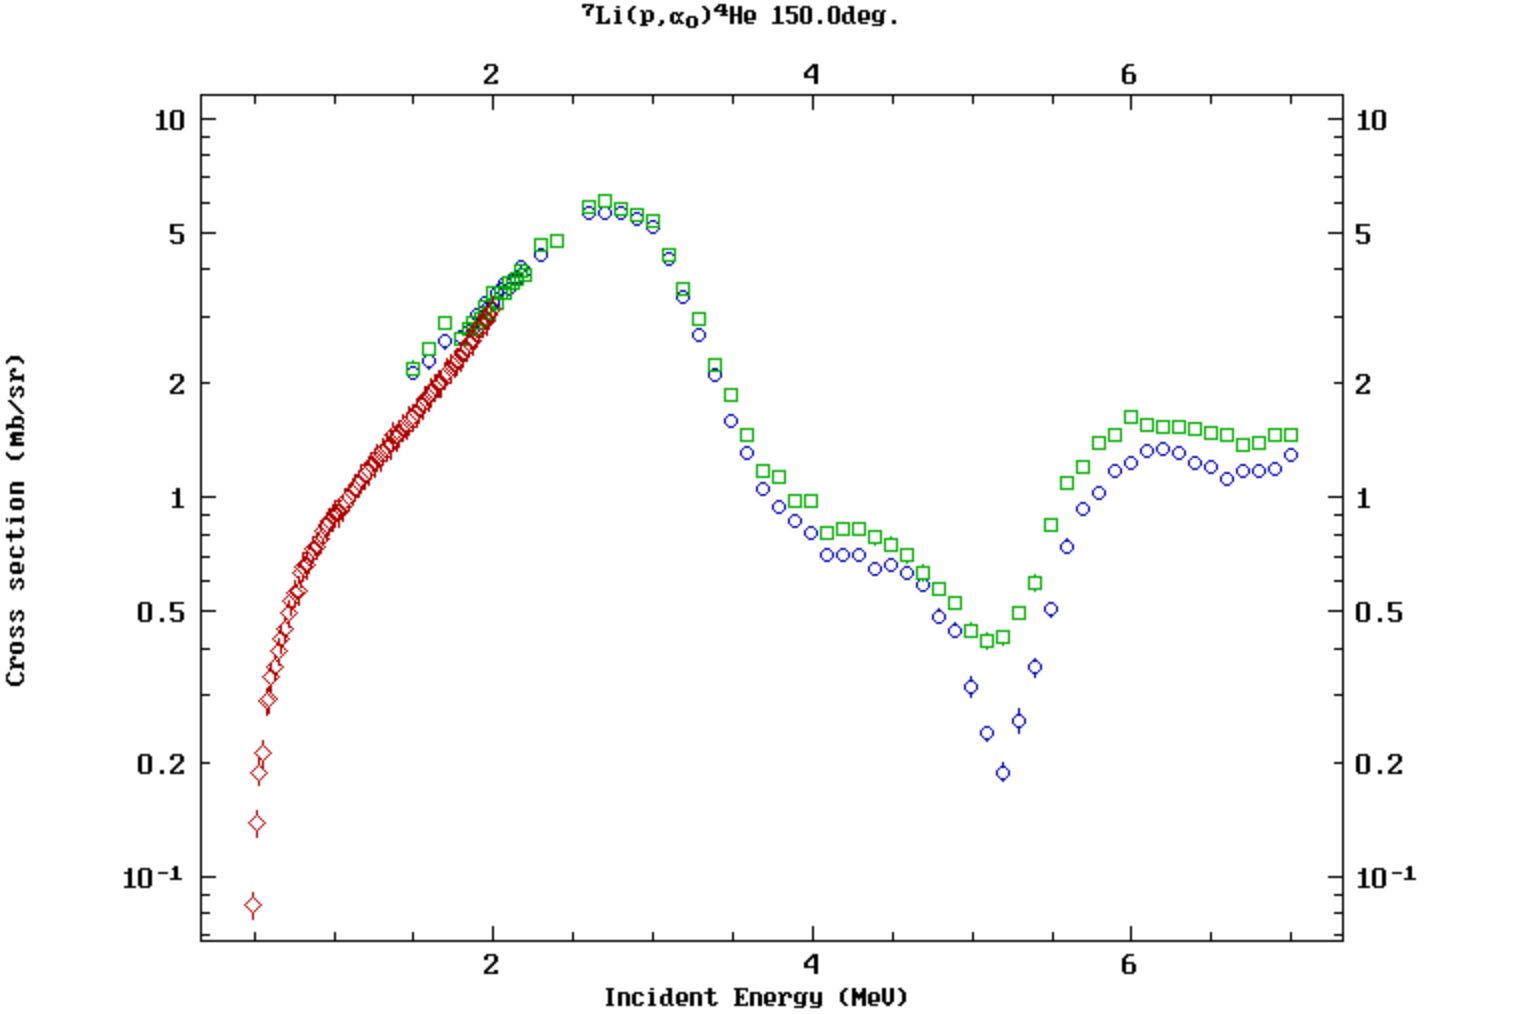
\includegraphics[width=0.95\linewidth]{../images/Li_crosssection_energy.jpeg}
  \captionof{figure}{Cross section of the reaction between protons and Li-7 as a function of the beam energy.}
  \label{crosssection}
\end{center}

We are only interested in the energy range of $[0.5,5]$ MeV because the energy of the beam is limited by the accelerator.
As we can see in figure \ref{crosssection}, the cross section of the reaction is maximum in the $[2.5,3]$ MeV range. 
Therefore, since we want to detect the Li-7 in the samples, we should choose the energy of the beam to be in this range.

\section{Safety considerations}

During the experiments, the accelerator will be producing a beam of protons with a kinetic energy of up to 5 MeV. Because of this there will be a high radiation level near the accelerator.
There are radiation maps that show the radiation levels in different areas of the laboratory and need to be strictly followed.

\section{Beamtime requested}

In order to complete our project we will need one full day of beamtime at the CTN laboratory \cite{IST}. Alongside this day, we will
also meet with the investigators at CTN for another two mornings to discuss the project, before the experiment and the
results after the experiment:

\begin{table}[H]
\centering
\begin{tabular}{|w{0.4\linewidth}|w{0.3\linewidth}|w{0.15\linewidth}|}
\hline
Phase & Date & Duration \\ \hline
Theoretical Background, Planning and Lab Overview & 30/11/2023 9h30 & 4h \\ \hline
Experiment & 7/12/2023 8h00 & 8h \\ \hline
Results Discussion & To be arranged & 4h \\ \hline
\end{tabular}
\end{table}

\section{Results expected}

We will obtain the energy spectrum of the alpha particles resulting from the reaction between the protons and the
samples. 
For the glass samples, we expect to see a profile due to the particles that come from different depths of the sample and
therefore have lost different amounts of energy. In the implant samples, we expect to see a peak at the energy corresponding
to the energy of the alpha particles produced by the reaction.
In both cases, the samples are composed by other types of atoms such as silicon and boron, which will also emit charged
particles. By obtaining the expected energy spectrums we can infer the presence of Li in the samples. If possible we will also try
to quantify the amount of Li present by analyzing the amount of energy deposited in the spectrums.

\paragraph*{Energy Values} The alpha particles are supposed to have the energies calculated in equation \ref{eq:energies} ($E_{\alpha_1}$ and $E_{\alpha_2}$). 
In the glass sample, we expect to see an energy profile before each peak and in the implant sample we only expect to see the peaks.

\paragraph{}

Other phenomena such as Rutherford Backscattering and Elastic Scattering are also expected to occur. These are responsible for energy peaks in both sample's spectra at lower than the expected energy values.

\section{Concluding remarks}

By identifying the presence of light isotopes at low energies ($<5$MeV), we achieve a practical method to evaluate the presence and the amount of these light isotopes in technological materials.
Until now, the only way to do this was through atomic spectroscopy, which, besides not being able to detect the presence of light isotopes, is a much more complex and expensive method.

\printbibliography
\nocite{*}

\end{multicols}

\end{document}